\documentclass[12pt]{article}
\usepackage{threeparttable}
%_ PACKAGES __________________________________________________________________________ %
	
    %__ INPUT/OUTPUT LANGUAGE _________________________________ %
    \usepackage[USenglish]{babel}
    \usepackage[utf8]{inputenc}
    \usepackage[T1]{fontenc}
    %\usepackage{indentfirst}

    %__ MATH __________________________________________________ %
    \usepackage{amsfonts}
    \usepackage{amssymb}
    \usepackage{amsmath}
    \usepackage{amsthm}
    \usepackage{bbm}
    
    %__ THEORY __________________________________________________ %
    \newtheorem{name}{Printed output}
	\newtheorem{lemma}{Lemma}
	\newtheorem{prop}{Proposition}
	\newtheorem{cor}{Corollary}
	\theoremstyle{definition}
	\newtheorem{definition}{Definition}

    %__ GRAPHS & TABLES________________________________________ %
    \usepackage{graphicx}
    \usepackage{subfig}
    \usepackage{booktabs}
    %\usepackage{multirow}
    \usepackage{array}
    \usepackage{caption}
    %\usepackage{subcaption}
    %\usepackage[flushleft,online,para]{threeparttable}
    
    %\usepackage{parskip}                       % WHAT IS THIS FOR?

    \usepackage{floatrow}
        \floatsetup[table]{style=plaintop}     % LEAVE TABLE CAPTIONS AT THE TOP
    %\usepackage[nolists,nomarkers]{endfloat}             % PUT FIGURES AT THE END OF DOCUMENT; DOESN'T WORK WITH \usepackage{float}

    \usepackage{tabularx}
        \newcolumntype{Z}{>{\centering\arraybackslash}X}
        \newcolumntype{L}{>{\raggedright\arraybackslash}X}

    \usepackage{dcolumn}
        \newcolumntype{d}[1]{D{.}{.}{#1}}

    \usepackage{rotating}                      % for **sideways**tables
    \usepackage{lscape}
    \usepackage{pdflscape}

    %__ BIBLIOGRAPHY __________________________________________ %
    \usepackage[round]{natbib}

    %__ PDF, DISPLAY & PRODUCTIVITY ___________________________ %
    \usepackage{xcolor}
        \definecolor{darkblue}{rgb}{0,0,0.4}
    \usepackage{hyperref}
        \hypersetup{
            colorlinks = true,
            linkcolor = darkblue,
            citecolor = darkblue,
            pdfborder = 0 0 0,
            pdfdisplaydoctitle = true,
            pdfhighlight = /N,
            pdfpagelayout = OneColumn,
            pdfpagemode = UseNone,
            pdfstartview = {FitH},
            pdfauthor = {{AB, CF \& JR}},
            pdftitle = {{DYN}},
            pdfsubject = {{}}
        }

    \usepackage[textsize=footnotesize, colorinlistoftodos, textwidth=4cm, obeyDraft]{todonotes}
    %\usepackage{fixme}
        % commands \fxnote; \fxwarnin; \fxerror; \fxfatal
        % \fxsomething{options}{note}{TEXT}* highlights the TEXT

    \usepackage{geometry}
        \geometry{verbose,tmargin=2.5cm,bmargin=2.5cm,lmargin=2.5cm,rmargin=2.5cm}
    \usepackage{setspace}
        \onehalfspacing

    \usepackage[bottom, multiple]{footmisc}    % keep footnotes at the bottom of the page, and allow for multiple footnotes at one place.

    \usepackage{verbatim}
    \usepackage[normalem]{ulem}     % strikethrough fonts
    \usepackage{mathpazo}

    %\usepackage{syntonly}       % if uncommented, this will prevent latex to produce
    %    \syntaxonly             %   any output. latex will only check for syntax.
    %\usepackage[displaymath,tightpage]{preview}
    %\graphicspath{{//graphs/}}

    %__ APPENDIX _____________________________________________ %
    \usepackage[toc,page]{appendix}

%__ COMMANDS _________________________________________________________________________ %
    \newcommand{\mc}{\multicolumn}
    \newcommand{\lbar}{\underline}
    \newcommand{\ubar}{\overline}




\title{\textbf{Can Monitoring and Transparency Make Food Safer? Examining Food Inspection Grading System in New York City}}

\author{Jason Huang}

\date{\bigskip \today}


% _ DOCUMENT _________________________________________________________________________ %

\begin{document}

\maketitle

\thispagestyle{empty} \newpage

\onehalfspacing \setcounter{page}{1}

%\maketitle

\textbf{Abstract}

Sanitation qualities of retail food establishments are a great public health concern. To incentivize restaurants to improve quality and increase transparency for consumers, many municipalities have made food inspection results public, releasing them online and/or requiring restaurants to post them on their windows. This project measures the the causal impacts of these transparency policies on consumer choices and restaurants? sanitation qualities. I investigate the impact of food inspections on restaurant cleanliness by estimating how inspection results affect subsequent inspection results and 311 complaint calls by customers. To deal with the endogeneity of the inspection results, I use the inspector-specific tendencies as an instrumental variable. I find that these individual tendencies are predictive not only of the overall inspection scores but also the specific violations that are cited, despite the random assignment process that results in similar restaurant characteristics across inspectors. The findings from this study have important implications for optimal design of the policy, especially as more states and cities prepare to launch their own targeted transparency regulations. 

\section*{Introduction}

Food hygiene at restaurants is a great public health concern. The CDC estimates that over 3 million incidents of food-borne illness occur in the US annually, with 60\% of the cases resulting from  dining in restaurants\footnote{Surveillance for Foodborne Disease Outbreaks United States: 2013 Annual Report. Available: https://www.cdc.gov/foodsafety/pdfs/foodborne-disease-outbreaks-annual-report-2013-508c.pdf}. Unlike food quality or service, which consumers can easily observe, food sanitation remains opaque to consumers since most diners cannot venture back to the kitchens and monitor the food preparation process. Local health departments have long conducted regular food inspections to ensure that restaurants meet certain hygiene standards. However, in the last two decades, major cities have implemented policies that make these inspection results public by requiring restaurants to post letter grades on their windows. In the case of New York City, starting from 2010, the Department of Health and Mental Hygiene (DOHMH) has required restaurants to post A, B, or C, depending on how many violations the food inspectors cited.

My dissertation studies the how New York City's food inspection grading system's by analyzing the two channels through which such target transparency policy can improve social welfare: demand side and supply side. For the demand side, these grades inform the customers so that they can avoid restaurants with poor food sanitation qualities. There is strong evidence that consumers respond to these posted grades. \cite{jie_leslie_05} and \cite{jie_leslie_09} combine inspection grades with tax revenue data and find evidence that consumer choices responds to the posted grades. Restaurants that enjoy upgrades see increases in revenues while places that suffer downgrades experience drops in revenues. I build on those studies by using a proprietary data on debit and credit card transactions, which allow me recover heterogenous effects across customers. 

For the supply side, having to post their food inspection results may incentivize restaurants to improve their overall cleanliness. However, the evidence on the supply side is more mixed. \cite{jie_leslie_05} and \cite{Simon_05} find strong evidence for decrease in hospitalization for foodborne illnesses in jurisdictions in Los Angeles following the enactments of the grading systems. A major shortcoming of using the number of foodborne illnesses is that it is a very noisy measure. Food poisoning often goes unreported and cannot easily be traced back to the original establishment. On the other hand, by using 311 complaint calls and Google Trend of search terms related to food poisoning as measures for sanitation conditions, \cite{Ho_2012} finds no evidence that rates of foodborne illnesses changed New York City instituted its grading system.  \cite{Wong_at_el_2015} and \cite{Meltzer_2015} use inspection scores to measure restaurant cleanliness. After finding that improved sanitation scores and lower violation fines following the reform, they conclude that the reform improved sanitation practices. However, because of the two studies' lack of comparable control groups, they cannot rule out the possibility that changes in other confounding factors led led to the observed changes in the variables of interest.  For instance, the amount of fine and the criteria associated with each violation changed after the reform, making scores across the two time periods difficult to compare. 

Rather than measuring the overall impact of the policy by making pre-post comparisons, I focus on the impact of the inspections on the hygiene qualities. Can we find evidence that restaurants improve by learning from the violations that were cited? Do stricter inspections lead to better compliance? The causal link between government monitoring and and compliance behaviors have been explored in other areas such as taxation \citep{Gemmell_Ratto_12} and \citep{Kleven_Waseem_13} and environmental protection \citep{Duflo_Greenstone_14}. \cite{Jin_Lee_12} also look at food inspections, but they focus on the inspectors' behaviors. A complication that makes this analysis non-trivial is that inspection results are endogenous, correlated with variables that are both hard to observe and drive the outcomes of interests. To overcome the endogeneity problem, I use inspector-specific tendencies as instrument for the inspection results. I provide more details in a later section.  

\section*{New York City Food Inspection and Grading System}

New York City's Department of Health and Mental Hygiene oversees the food safety program. It sends out food inspectors to restaurants to conduct inspections. Each restaurant receives at least one inspection a year. Starting in 2005, the city implemented a numerical scoring system. It outlined ninety-eight violations, broken into eight categories: food temperature, food source (general and critical), food protection, facility design, personal hygiene, vermin/garbage, and facility maintenance. Each violation is associated with a range of scores, and the inspector assigns the numerical score that reflects the severity of the violation. The sum of the individual scores exceeding certain threshold triggers either re-inspections or closure of the restaurant. 

Starting in 2010, the sum of the scores were converted to letter grades, A, B, C, based on specified cutoffs. In addition, the city required the restaurants to post these letter grades on the entrance so that they are clearly visible to the customers. The grading policy also changed the inspection cycles. It introduced dual inspection cycles, which involved the a random initial inspection and a possible re-inspection within a month if the initial inspection results in a letter grade lower than an A. Inspectors to both cycles are randomly assigned so rarely do the same inspector inspector a restaurant twice in a roll. Finally, the time between an initial inspection and the subsequent initial inspection depended on the inspection results from the original inspection. If the initial inspection results in an A, the subsequent inspection occurs in roughly a year but if it results in a C, the subsequent inspection occurs after between 90 to 150 days. 

\section{Data}

\subsection{Food Inspection Data}

\begin{figure}[h]
\centering
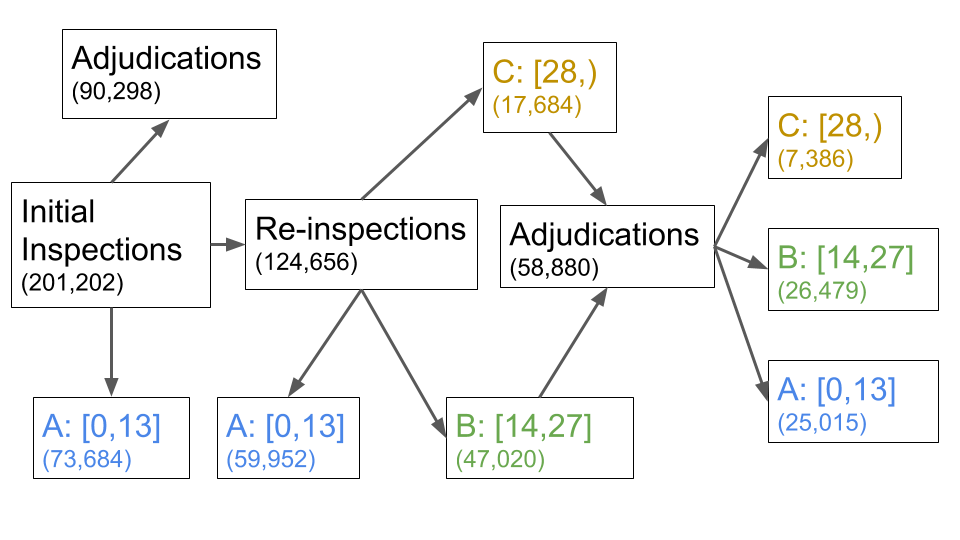
\includegraphics[scale = 0.4]{Scores.png}
\caption{T}
\end{figure}
\subsection{311 Calls}

I also use the frequency of 311 calls to assess the hygiene qualities of the restaurants. [Describe what 311 calls are]

[Basic Description of the Data]

[Matching Process]

\section{Empirical Strategies}

\subsection*{Inspector Assignment}


I study the second channel -- the supply side -- by measuring how a restaurant's inspection results affect subsequent inspection performances. Do restaurants that received lower grades improve? Do restaurants that did well slack off and perform worse? Do restaurants shift attention toward areas that they have done poorly in the past at the expense of areas in which they have done well in previous inspections? I answer these questions by analyzing the panel data of over 300,000 food inspection results conducted by over 250 inspectors and across over 50,000 restaurants from 2010 to 2016. I then combine this data with 311 call data to DOHMH. New York City's 311 phone line is a centralized line for residents to call city agencies and services about non-emergency issues. These calls include complaints about food poisoning or unsanitary practices at retail food establishments. Each call records the date and the address of the incidence, along with the type of complaints. 

Two critical components of my empirical strategy are the random assignment of food inspectors and the different levels of leniency across inspectors. These two factors allow me to use inspector fixed effects as an instrumental variable for each inspection result\footnote{Other papers that use the random assignments of judges, inspectors, or reviewers to estimate the causal impact of government policies include \cite{Doyle_07, Doyle_08} and \cite{Maestas_13}.}. To better illustrate this point, consider the thought experiment of two identical restaurants, with one randomly assigned a strict inspector and who assigns a poor grade and the other assigned a lenient inspector who assigns a good grade. Because of the randomness of the inspector assignments, we can use the difference in the observed outcomes between the two restaurants as the causal impact of the inspection results. Finally, since the inspections are conducted once a year, the food inspection data also tracks the survival rate of restaurants across time. Combining this with the empirical strategy I described above also allows me to answer whether this policy has hurt local businesses. 

\subsection*{Policy Implications}

Mandatory disclosure has become become a popular regulatory tool to improve product qualities and ensure consumer safety. But we need empirical studies to measure the magnitude of these policies' intended consequences and test for the presence of unintended ones. Furthermore, a comprehensive understanding of the NYC’s food inspection system on both the consumers and suppliers has important policy implications beyond the city. As more states and other cities\footnote{Seattle launched its grading system in January 2017. This article describes a survey the county sent out that asked residents for their feedback on the best design of the grade cards: http://www.seattletimes.com/seattle-news/health/smiley-faces-for-food-safety-king-county-gears-up-for-new-restaurant-grading-system/} prepare to launch their own restaurant hygiene grading systems, the findings from my projects can offer guidance on the optimal design of these programs. 

\newpage

\bibliographystyle{apa}

\bibliography{Biblio}



\end{document}
The main resource from IRISS that I'd like to access is Sherlock GPU. My data set contain over 500,000 inspections, and for each inspection, I have up to 80 different types of violations. For certain regression, specification, I may have over 10's of millions of observation, and being able to use the GPU will allow faster computation that allows me to experiment with more empirical specifications. 

I supplement the literature by my choice of outcome variables and my methodology. While I also use results from food inspections as measures for restaurant cleanliness, I exploit the randomness of inspector assignments to estimate the causal impact of third-party monitoring on subsequent compliance behaviors

My study also fits in with a broader principal-agent literature that examines the interaction between government regulations and compliance behaviors. For example, \cite{Duflo_Greenstone_14} study how increased frequencies of environmental inspections influence pollution from plants. \cite{Gemmell_Ratto_12} and \cite{Kleven_Waseem_13} measure the impact of tax audits on tax non-compliance behaviors.

These policies for better transparency have the potentials to improve social welfare through two channels: demand side and supply side. For the demand side, these grades inform the customers so that they can avoid restaurants with poor food sanitation qualities. There is strong evidence that consumers respond to these posted grades\footnote{\cite{jie_leslie_05} and \cite{jie_leslie_09} combine inspection grades with tax revenue data and find evidence that consumer choices responds to the posted grades. Restaurants that enjoy upgrades see increases in revenues while places that suffer downgrades experience drops in revenues.}. For the supply side, having to post their food inspection results may incentivize restaurants to improve their overall cleanliness. However, the evidence on the supply side is more mixed\footnote{\cite{jie_leslie_05} and \cite{Simon_05} find strong evidence for decrease in hospitalization for foodborne illnesses in jurisdictions in Los Angeles following the enactments of the grading systems. On the other hand, by using 311 complaint calls and Google Trend of search terms related to food poisoning as measures for sanitation conditions, \cite{Ho_2012} finds no evidence that rates of foodborne illnesses changed New York City instituted its grading system.}\footnote{A major shortcoming of using the number of foodborne illnesses is that it is a very noisy measure. Food poisoning often goes unreported and cannot easily be traced back to the original establishment. Instead, \cite{Wong_at_el_2015} and \cite{Meltzer_2015} use inspection scores to measure restaurant cleanliness. After finding that improved sanitation scores and lower violation fines following the reform, they conclude that the reform improved sanitation practices. However, because of the two studies' lack of comparable control groups, they cannot rule out the possibility that changes in other confounding factors such as food sanitation standards following the reform led to the observed changes in the variables of interest. 
}. Opponents of these policies, however, have pointed out that they pose unnecessary compliance costs and hurt local businesses. 
